
%%%%%%%%%%%%%%%%%%%%%%%%%%%%%%%%%%%%%%%%%%%%%%%%%%%%%%%%%%%%%%%%%%%%%%%%
% Approach
%%%%%%%%%%%%%%%%%%%%%%%%%%%%%%%%%%%%%%%%%%%%%%%%%%%%%%%%%%%%%%%%%%%%%%%%
\section{Proposed Approach}
\label{sec:method}

\note{This intro here must be much more concrete, it is too general and high level. Also, it is very long.}

% \begin{figure}[t]
% \centering
% 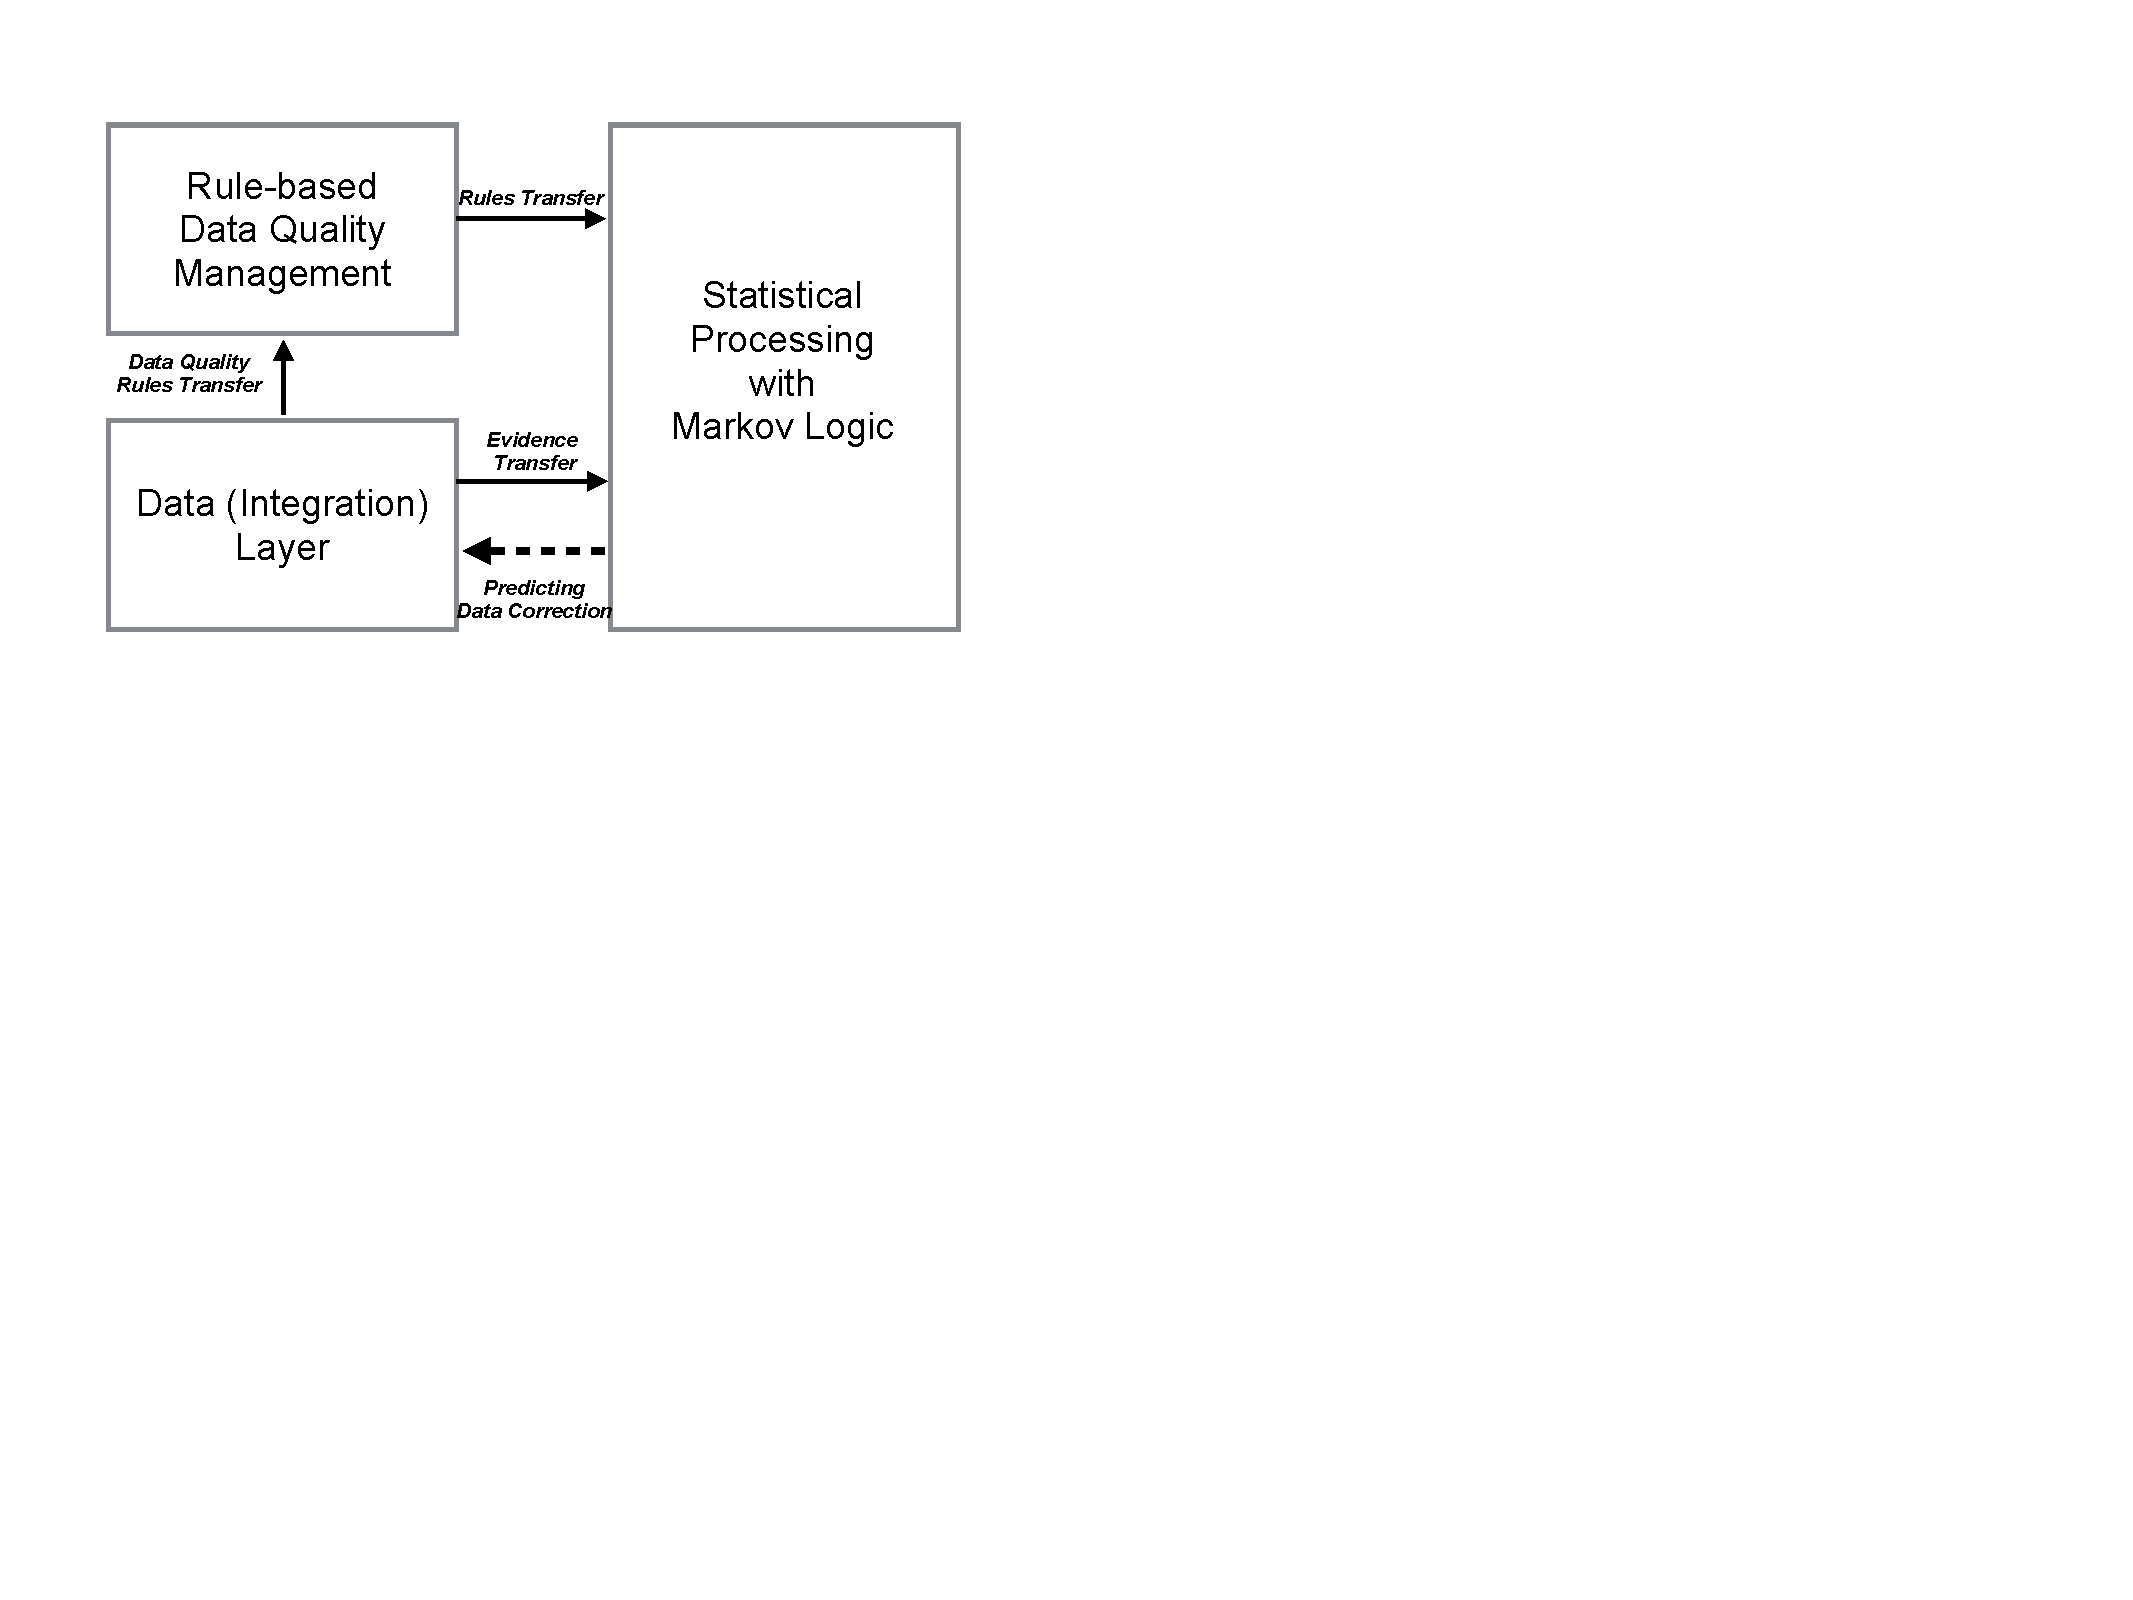
\includegraphics[width=200px, height=140px]{img/system.pdf}
% \caption{\anno{Rmove this picture?} Our proposed method for data cleaning based on Markov logic consists of three main components: 
% (I) A \textbf{Rule-based Data Quality Management} component that is based on the data quality rules to address different data quality issues;
% (II) A \textbf{relation prediction} component based on probabilistic inference performed by the Markov logic framework and (III) 
% a \textbf{Data Layer} that includes a number of data sources including relational and semi-structured data.}
% \label{fig:system}
%\end{figure}     

Our proposed approach is to model data cleaning rules in a Markov Logic~\cite{domingos2009markov} formalism and use probabilistic inference 
for data cleaning. \anno{CAN WE USE WORKFLOW HERE? (L.V)
\begin{inparaenum}[\itshape I\upshape)]
\item a Rule-based Data Quality Management component;
\item a Statistical Inference with Markov Logic component; and
\item the Data Layer.
\end{inparaenum}}

We see the following advantages in applying Markov Logic for data cleaning: First, in order to infer the types of errors and their sources, we consider integrity constraints to be probabilistic. We build on an existing approach to specify \textit{"soft"} functional dependencies between columns~\cite{Ilyas:2004:CAD:1007568.1007641} \anno{so its not a contribution of your work?}.  We use the notion of \textit{"soft"} FDs, where one attribute determines the value of the another attribute in a probabilistic way, as a basis for modeling Markov Logic Networks. In other words, if no perfect resolution of a rule-set is possible, we may be interested in finding data cleaning steps that fulfill as many rules as possible while violating only a few~\cite{genesereth1987logical}. 

 For example, we denote all key constraints based FDs as \textit{hard} rules~\cite{bertossi2011database} \anno{How does this apply to our running example?}. Second, one of the challenges while applying machine learning for repairing errorneous data over-fitting \anno{You need to explain overfitting!}. This problem becomes apparent when modeling data quality rules that hold only for a fraction of data, but do not hold globally. Markov logic programs with \textit{"soft"} rules prohibit over-fitting by adding weights to the constaint-based rules \note{big claim, do you have a reference?}. \anno{HOW DOES THIS RELATE TO THIS PAPER? Third, Markov logic facilitates the incorporation of rich domain knowledge for data with relational structure or dependencies between attibutes (also called non-i.i.d. models~\cite{spies2013knowledge})} and allows us to perform joint inference over several interleaved hidden predicates. By making use of this joint inference and soft rules we show that we can improve data cleaning performance over other data cleaning systems \anno{be concrete, what do you mean exactly? accuracy? runtime?}. Furthermore, we show that we are not limited to functional dependencies as data quality rules, but rather are able to define arbitrary rules as long as they are expressible as weighted first-order logic \anno{where exactly do you show that? how does this help with data cleaning?}. For instance, within the Markov logic program one can define both positive and negative data cleaning rules. Markov logic as a formalism is independent of the inference engine. This means that we can exchange the method of joint inference used for data repair prediction as suits our needs. For instance, in this work we use an Integer Linear Programming optimization for \textsc{map} (maximum a-posteriori) inference~\cite{NoessnerNS13}. \anno{Why do we want that? What is the advantage?}
    
In the following, we illustrate how to transfer data cleaning rules into Markov Logic and leverage probabilistic inference to determine data repair operations for a given dataset. 

%\begin{figure*}[t]
% \centering
% 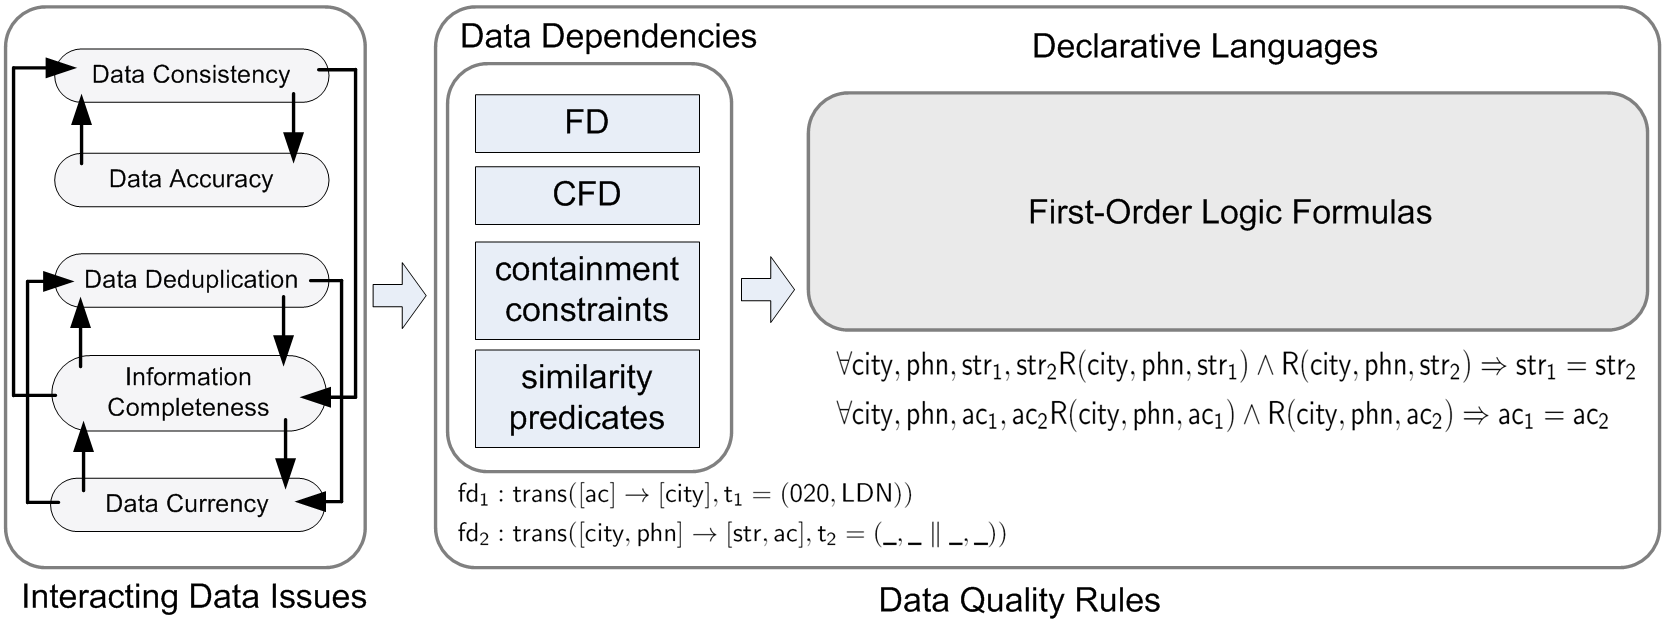
\includegraphics[width=500px, height=180px]{img/Grafik-2.png}
% \caption{System Overview: Component (I), the \textbf{Rule-based Data Quality Management} component, is based on the data quality rules 
% that address different data quality issues.}
% \label{fig:system1}
%\end{figure*}


%\begin{figure}[t]
 %\centering
 %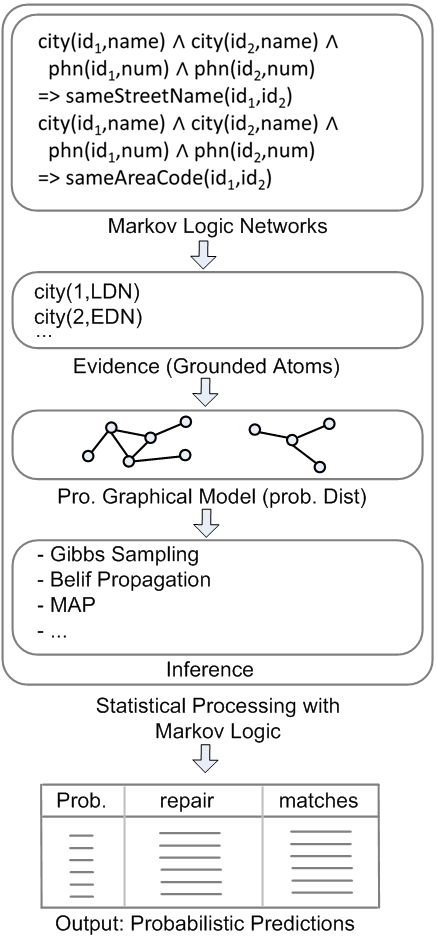
\includegraphics[width=160px, height=320px]{img/Grafik-3.png}
 %\caption{System Overview: Component (II), the \textbf{Statistical Processing} component, is based on probabilistic inference performed 
 %by the Markov Logic framework.}
 %\label{fig:system2}
%\end{figure}

\begin{figure*}[t]
 \centering
 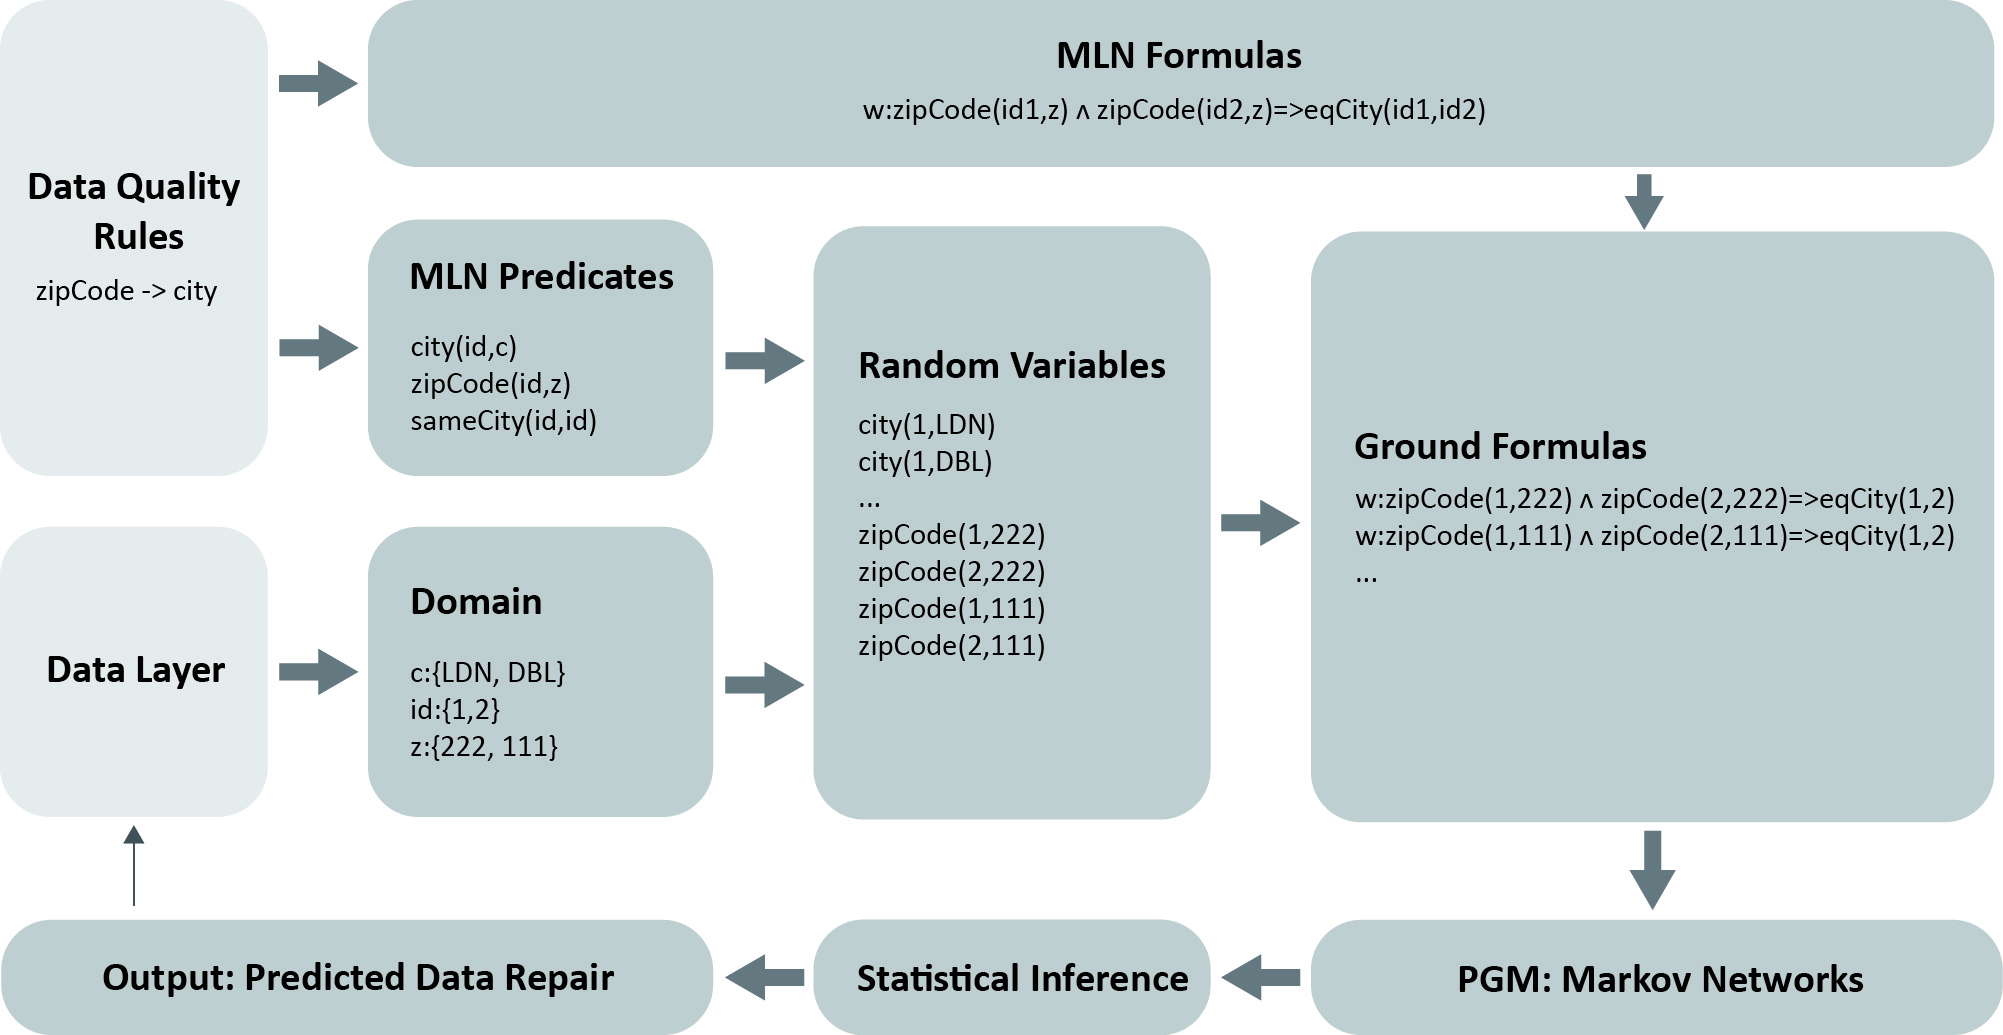
\includegraphics[width=450px, height=200px]{img/mlogic-grounging.jpg}
 \caption{Markov Logic Network grounding process constists of two phases 1) MLN definintion by fixing MLN schema, domain and weighted formulas; 2) MLN instantiation by assigning truth values to the all possible instantiations of the MLN predicates and using these ground atoms in formulas.}
 \label{fig:mlngrounding}
\end{figure*}

\begin{table}[t]\footnotesize
\scriptsize
\centering
\begin{tabular}{@{}ll@{}}
\toprule
Phase                                                                             & Example                                                                                                                                                          \\ \midrule
1) Schema definition                                                              & \begin{tabular}[c]{@{}l@{}}$t_2$(item, fn, ln, st, city, zip, tel)\end{tabular}                                                              \\ \midrule
\begin{tabular}[c]{@{}l@{}}2) Observed predicates \\ MLN declaration\end{tabular} & \begin{tabular}[c]{@{}l@{}}$\mathsf{\textsf{firstname}(id, value)}$ \\ $\mathsf{\textsf{lastname}(id, lastname)}$ \\ $\mathsf{\textsf{street}(id, street)}$ \\ $\mathsf{\textsf{city}(id, city)}$\\ $\mathsf{\textsf{zip}(id, code)}$ \\ $\mathsf{\textsf{phone}(id, num)}$\end{tabular} \\ \midrule
3) Data                                                                           & \begin{tabular}[c]{@{}l@{}}$t_2$(Galaxy 5, NULL, Miller, \\ 12 Hay St., NULL, 818, 11234)\end{tabular}                                                              \\ \midrule
4) Grounded (evidence) atoms                                                      & \begin{tabular}[c]{@{}l@{}} $\mathsf{\textsf{item}(2, Galaxy5)}$ \\ $\mathsf{\textsf{lastname}(2, Miller)}$ \\ $\mathsf{\textsf{street}(2, 12HaySt.)}$ \\ $\mathsf{\textsf{zip}(2, 818)}$ \\ $\mathsf{\textsf{phone}(2, 11234)}$\end{tabular}                         \\ \bottomrule
\end{tabular}
\caption{\label{tab:mlndeclare} MLN declaration process and creation of grounded atoms for tuple 2 in the \textsc{Transactions} example table.}

\end{table}


\subsection{Data Cleaning Rules as Markov Logic}
\label{sec:ml}
We define data cleaning rules in the form of CFDs and MDs as introduced in Section~\ref{sec:expl}. For example, given the following functional dependency $\phi: X \rightarrow Y$ where $X \subseteq attr(\mathcal{R}) $ and $Y \subseteq attr(\mathcal{R}) $ are subsets of $\mathcal{R}'s$ attributes $attr(\mathcal{R})$. According to the~\cite{Fagin:1982:HCD:322344.322347}, $\phi$ can be expressed as \textit{first-order logic} sentence:
\begin{equation}
\mathsf{\forall x, y_1, y_2, z_1, z_2 \mathcal{R}(x, y_1, z_1) \wedge \mathcal{R}(x, y_2, z_2) \Rightarrow y_1=y_2}
\label{fd2fol}
\end{equation}

This first-order logic sentence is crucial for compilation of data cleaning rules into predictive models \note{why do we need this intermediate step of first-order logic? explain}. In order to specify an MLN to solve data cleaning problem we first specify data quality rules, and subsequently translate them into Markov logic. As described previously, the base of the Markov logic is predicate calculus \anno{Where have you described that?}. Therefore, one important step is the generalization of the compilation from the formal constraint based data cleaning rules into the predicate calculus \note{Why?}.

\anno{What do you mean with components and sentences here? You start to introduce another terminology out of nothing. This is superconfusing!}
Consider data quality rule $\phi$ as a composite component, consisting of subcomponents such as atomic sentences (attribute), logical and quantified sentences (RHS and LHS of the rule). To describe the structure of $\phi$ in a predicate calculus, we need to choose symbols that designate the elements of our conceptualization. In the following we define the \textit{vocabulary} we use for data quality rules: \anno{WHY ANOTHER VOCABULARY? THIS IS SUPER CONFUSING!!! REWRITE THIS PART TO CONNECT TO THE REST OF THE PAPER}

\begin{description}
	\item[Universe of Disclosure] is specified by the set of all objects from domain $dom(U)$ that is fixed for the set of attributes $attr(\mathcal{R})$.
	\item[Terms] A \textit{term} is used as a name for an object in the universe of discourse. We define \textit{variables} to denote arguments in atoms and \textit{constants} to denote data constants of particular domain $dom(U_i)$ of an $i$-th attribute $U_i \in attr(\mathcal{R})$.
	\item[Atoms] To designate the tuple in relation $\mathcal{R}$: $\mathcal{R}(x_1,x_2, \dots , x_n)$, we use atomic sentences $\mathsf{\textsf{attr-X}_1(id,v_1)}$, $\mathsf{\textsf{attr-X}_2(id,v_2)}$ $\dots$\\ $\mathsf{\textsf{attr-X}_n(id,v_n)}$ where $\mathsf{\textsf{attr-X}_i(id,v_i)}$ means that $\mathsf{v_i}$ is a attribute value of the $i$-th attribute in $\mathcal{R}(x_1,x_2, \dots , x_n)$ of the $id$-th tuple in relation $\mathcal{R}$.
	\item[Relation Constants]  which denote relations between several objects:
	\begin{itemize}
		\item Similarity: $\mathsf{\textsf{similar}(x_1,x_2)}$ means that $\mathsf{x_1}$ similar to $\mathsf{x_2}$ (e.g by using different similarity measures like cosine or jaccard similarities).
		\item Equality: $\mathsf{\textsf{equal-X}(id_1, id_2)}$ means that the values of the attribute X of two tuples $\mathsf{id_1}$ and $\mathsf{id_2}$ should be equal.
		\item Matching: $\mathsf{\textsf{match-X}(id_1, id_2)}$ means that values of two tuples $\mathsf{id_1}$ and $\mathsf{id_2}$ of the attribute X are identified to match.
	\end{itemize}
\end{description}

\note{Is the compilation more than a slightly different syntax? What are the challenges? This is one of the contributions, need more elaboration.} Given this vocabulary, we describe our conceptualization of the data quality rules with predicate-calculus sentences. For example, given the following functional dependency $\phi: X \rightarrow Y$ and the first-order logic sentence in Formula \ref{fd2fol}, the coresponding Markov logic formula is compiled as follows:
\begin{flalign*}
  & \mathsf{\textsf{attr-X}(id_1, x) \wedge \textsf{attr-X}(id_2, x) \Rightarrow \textsf{equal-Y}(id_1, id_2)} & 
\end{flalign*}
\vspace*{-0.5cm}

Using similar approach the matching dependency $ \mu: \mathcal{S}_1[x_1]\approx \mathcal{S}_2[x_2]\rightarrow \mathcal{S}_1[y_1]\rightleftharpoons \mathcal{S}_2[y_2]$ on a database instance $\mathcal{D}$ with two relational schemas $\mathcal{S}_1$ and $\mathcal{S}_2$ is translated as follows:
\begin{flalign*}
  & \mathsf{\textsf{attr-X/S1}(id_1, x_1) \wedge \textsf{attr-X/S2}(id_2, x_2) \wedge \textsf{similar}(x_1, x_2)} & \\
  & \mathsf{\Rightarrow \textsf{S1/match-Y/S2}(id_1, id_2)} & 
\end{flalign*}
\vspace*{-0.5cm}

In case, the matching dependency is specified by using two relations, the according attributes are marked with its containing relation $\mathsf{\textsf{attr-X/}}\mathcal{R}$. Furthermore, as introduced above, we use the following predicates to represent operators in the data quality rules like:

\begin{table}[h]\footnotesize
\scriptsize
\centering
\begin{tabular}{@{}lcl@{}}
\toprule
Concept    & Operator & Predicate \\ \midrule
Similarity & $\mathcal{S}_1[x_1]\approx \mathcal{S}_2[x_2]$        & $\mathsf{\textsf{similar}(x_1,x_2)}$ \\
Equality   & $y_1=y_2$ & $\mathsf{\textsf{equal-Y}(id_1, id_2)}$ \\
Matching   & $\mathcal{S}_1[y_1]\rightleftharpoons \mathcal{S}_2[y_2]$   & $\mathsf{\textsf{S1/match-Y/S2}(id_1, id_2)}$ \\ \bottomrule
\end{tabular}
\end{table}

\anno{TOO GENERIC AND HIGH LEVEL, SOUNDS LIKE A COPY FROM AN ML TEXTBOOK. CONNECT THIS TO OUR PROBLEM!
MLNs are created by writing a set of first-order logic rules with weights, constructed using variables 
that range of objects in the domain of interest and predicates that represent relations between these objects.
Predicates can be observed or hidden. \textit{Observed predicates} are relations between objects that can be seen in a
given data set. $\mathsf{\textsf{attr-X}_1(id,v_1)}$, $\mathsf{\textsf{attr-X}_2(id,v_2)}$ $\dots$ $\mathsf{\textsf{attr-X}_n(id,v_n)}$  where $\mathsf{\textsf{attr-X}_i(id,v_i)}$ are observed predicates. In addition, an MLN may have a number of \textit{hidden predicates}, meaning that they are not observed in the input data, but can be inferred through rules. In our case, $\mathsf{\textsf{equal-Y}(id_1, id_2)}$ and $\mathsf{\textsf{S1/match-Y/S2}(id_1, id_2)}$ are hidden.  The goal of probabilistic inference is to infer the likelihood for observed and hidden predicates given a rule set and evidence. We define the MLN in such a way that reasoning about hidden predicates given evidence and data cleaning rules allows us to determine data repair operations.}

%\subsubsection{First-Order Logic Formulae}
\note{Explain why we are doing all of this? What is the advantage?}
To demonstrate the first-order syntax, consider the following CFD from the motivation example in Section~\ref{sec:expl}, which states that if any two tuples agree on attribute values for $\mathsf{\textsf{city}}$ and $\mathsf{\textsf{phone}}$, then the attribute values on $\mathsf{\textsf{street}}$ and $\mathsf{\textsf{zip}}$ should agree as well:
\begin{equation*}
\mathsf{fd: \textsc{transaction}([\textsf{city}, \textsf{phone}] \rightarrow [\textsf{street}, \textsf{zipcode}])}
\end{equation*}
\vspace*{-0.5cm}

We assume that CFDs are provided in the normal form. This means if $\psi(X \rightarrow Y_1,Y_2,\dots , T_p)$, then $\psi$ will be decomposed into several CFDs where $RHS(\psi)$ (right hand side of $\psi$) becomes a single attribute: $\psi_1(X \rightarrow Y_1 , T_p)$, $\psi_2(X \rightarrow Y_2 , T_p) \dots$. Following the normalization rule for functional dependencies, we split the $\mathsf{fd}$ rule into two:
\begin{flalign*}
& \mathsf{cfd_1: \textsc{transaction}([\textsf{city}, \textsf{phone}] \rightarrow [\textsf{street}], t_1=(\_, \_ \parallel  \_))}& \\
& \mathsf{cfd_2: \textsc{transaction}([\textsf{city}, \textsf{phone}] \rightarrow [\textsf{zipcode}], t_2=(\_, \_ \parallel  \_))}&
\end{flalign*}
\vspace*{-0.5cm}

According to~\cite{Fagin:1982:HCD:322344.322347} these $\mathsf{cfd_1}$ and $\mathsf{cfd_2}$ can be represented as the following two first-order logic formulae:
\begin{flalign*}
& \mathsf{1)~\forall~\textsf{city}, \textsf{phone}, \textsf{street}_1, \textsf{street}_2 }& \\
& \mathsf{\textsc{transaction}(\textsf{city}, \textsf{phone}, \textsf{street}_1)~\wedge~\textsc{transaction}(\textsf{city}, \textsf{phone}, \textsf{street}_2) }& \\
& \mathsf{ \Rightarrow \textsf{street}_1=\textsf{street}_2 }& \\
& \mathsf{2) ~\forall~\textsf{city}, \textsf{phone}, \textsf{zip}_1, \textsf{zip}_2 }& \\
& \mathsf{ ~\textsc{transaction}(\textsf{city}, \textsf{phone}, \textsf{zip}_1) \wedge~\textsc{transaction}(\textsf{city}, \textsf{phone}, \textsf{zip}_2) }& \\
& \mathsf{ \Rightarrow \textsf{zip}_1=\textsf{zip}_2 }&
\end{flalign*}
\vspace*{-0.5cm}

In words, the formulas state that if two tuples of the \textsc{transaction} relation agree on the \textsf{city} and \textsf{phone} values, then their \textsf{street} and \textsf{zip} values should be the same. In this paper we assume that these dependencies already determined by using methods reviewed in \cite{liu2012discover} or specified by domain experts manually. \anno{How does this affect the usability of the system?}

%\subsubsection{Markov Logic Compilation}

Once we have formulated our integrity constraints as first-order logic formulae, they can be translated into a Markov
Logic syntax. We illustrate this with the first-order logic formulae $\mathsf{cfd'}$ and $\mathsf{cfd''}$ from the previous section \anno{can't find them}:
Given that every attribute from the schema $\mathsf{\textsc{transaction}}$ is expressed as a predicate, we declare two observed predicates, 
namely $\mathsf{\textsf{city}(id, city)}$ and $\mathsf{\textsf{phone}(id, phone)}$. They indicate the values for the fields \textsf{city} and
\textsf{phone} for each tuple, given by its id. The full example is given in Table~\ref{tab:mlndeclare}, which shows how a tuple from the example database is translated into grounded atoms. 

In addition, we define two hidden predicates for our data quality rule, namely $\mathsf{\textsf{equal-street}(id, id)}$ and $\mathsf{\textsf{equal-zip}(id, id)}$. These predicates constitute our Markov Logic model \anno{??? that reflects $\mathsf{fd}$ rule above:}
\begin{flalign*}
	& \mathsf{1)  \textsf{city}(id_1, city) \wedge \textsf{city}(id_2, city) \wedge \textsf{phone}(id_1, phone) }& \\ 
	& \mathsf{  \wedge \textsf{phone}(id_2, phone) \Rightarrow \textsf{equal-street}(id_1, id_2)} & \\
	& \mathsf{2)  \textsf{city}(id_1, city) \wedge \textsf{city}(id_2, city) \wedge \textsf{phone}(id_1, phone) }& \\ 
	& \mathsf{  \wedge \textsf{phone}(id_2, phone) \Rightarrow \textsf{equal-zip}(id_1, id_2)} & 
\end{flalign*}
\vspace*{-0.5cm}

Please note that using the same argurments in predicates $\mathsf{\textsf{city}(id, city)}$ and $\mathsf{\textsf{phone}(id, phone)}$ encodes equality of the corresponding values in Markov logic program. 

Applying the normalization for functional dependencies, we model the $\mathsf{fd}$ consistency rule as two formulas in Markov Logic. 
Note that two different tuples are distinguished by $\mathsf{id_1}$ and $\mathsf{id_2}$. 
The data quality rules are the basis for MLN construction. The MLN itself is a template for a probabilistic graphical model. It constructs the probability distribution over all possible predicates in the MLN. A particular advantage of Markov Logic is its \textit{modularity} while modeling. This means that one can create "complex" statistical models by utilizing various "atomic" models. We consider each declared data quality rule as an "atomic" probabilistic model
(function). Together these small models form a "compound" model. Having declared the data quality rules by capturing all correlations and
constraints, we are able to write the MLN and perform the inference for the potential predicates. \note{DESCRIBE EXACTLY HOW WE DO THAT: In other words, we are able to predict the possible data quality issues such as inconsistency, missing values, values duplicates etc. }
\todo[inline]{each data cleaning rule is an atomic model; holistic treatment through the joint inference over the all atomic models.}

In the example above, we also declared two hidden predicates, one of which is $\mathsf{\textsf{equal-street}(id, id)}$. This predicate holds the information about possible repairs 
on the attribute $\mathsf{\textsf{street}}$ in the \textsc{transactions} tables in our running example from Section~\ref{sec:expl}.
Reasoning about such hidden predicates allows the system to decide what attribute gets a particular repair and what records are potential matches. 
Handling inclusion dependencies (IND) \anno{What are inclusion dependencies???} was studied in \cite{bohannon2005cost}, although we have not conducted any experiments on the INDs, we claim to be able to model INDs in a similar manner as they can be represented in first-order logic: $\mathsf{\forall x, y\mathcal{R}(x, y) \Rightarrow \exists z~\mathcal{S}(y, z)} $ and therefore being directly represented in Markov Logic.

So far we have shown how to express integrity constraints in terms of observed and hidden predicates. These rules are data agnostic~\cite{fan2012foundations}. In order to clean a data set with these rules, we need to ``ground'' these predicates with the available evidence, i.e. the database to be processed. We take the content of the database (a set of tuples) and produce a set of observed predicates. Each attribute value of the tuple is converted into an grounded atom. Assuming that $n$ is the number of schema attributes, each tuple from the database is converted into $n$ different Markov Logic evidence atoms.

For example, we translate transaction 2 in our running example into the following 6 grounded atoms: \textsf{item}(2, Galaxy 5), \textsf{firstname}(2, Max), \textsf{lastname}(2, Miller), \textsf{street}(2, 12 Hay St.), \textsf{zip}(2, 818) and \textsf{phone}(11234). These are examples of observed predicates for the data set. 

\subsection{Data Repair as Joint Inference}
%\todo[inline]{Manu: there is an example there.. so explain that with some probabilistic formulae and the corresponding PGM drawn out}
\anno{REMOVE AND REPLACE WITH A SINGLE SENTENCE: The main advantage of Markov logic is the ability to reason about complex and interacting relationships, such as different data quality issues. The query computation is also known as \textit{inference}. In addition, through the cleaning rules that we have defined in the Rule-based Data Quality Management component of our system, there are a number of hidden predicates we use for data repair. The Statistical Processing component of our system (see Figure~\ref{fig:mlngrounding} for an overview) executes probabilistic 
inference to determine probable groundings for the hidden predicates. This component takes as input both the Markov Logic Networks defined through component I, as
well as the grounded atoms produced by component III from the available data. It then constructs a probabilistic graphical model using these inputs on top 
of which it performs probabilistic inference. Figure \ref{fig:mlngrounding} visualizes the MLN grounding process.}

\anno{Where are we introducing more and more terminology? What are literals?} Given an MLN that models data cleaning rules, let $q \in \mathcal{L}^n$ denote a hidden predicate with $n$ \emph{literals} (random variables) $L_1,...,L_n$, where each literal $L_i$
has $2$ discrete states, $L_i = \lbrace 0,1 \rbrace$.
Then, the MLN is a joint distribution on  $L_1,...,L_n$ that 
is specified by a vector $\phi(q)$ of $d$ integer values, where
each element represents the number of true groundings of the 
corresponding literal in the formula and $d$ denotes the 
maximum number of literals in a given formula. Additionally, 
we have a weight/parameter vector $\theta \in \mathcal{R}^d$:
%\vspace{-3em}
\begin{equation*}
Pr \left( q | \theta \right) = 
\frac{1}{Z(\theta)} \exp\left( \langle \theta, \phi(q) \rangle  \right), 
Z(\theta) = \sum_{q \in \mathcal{L}^n}\exp\left( \langle \theta, \phi(q) \rangle  \right) 
\end{equation*}
%\vspace{-2em}
where $\langle \theta, \phi(q) \rangle$ denotes a dot product. 
$Z(\theta)$ is the normalization constant also called the 
\emph{partition function}. Since the partition function is a constant and the exponential is monotonic, finding the MAP assignment in our data cleansing problem is equivalent to finding the assignment $q_M$ that maximizes the probability $Pr \left( q | \theta \right)$.

The output of the inference are data repair operations; for example, the hidden predicate \textsf{equal-street} we defined in the previous section
may be determined by the system to have among other groundings the following likely value: $\mathsf{\textsf{equal-street}(1, 3)}$, indicating that
the \textsf{street} field for transaction 3 should have the same value as the \textsf{street} field of transaction 1. 
In this case, the data repair operation is to replace the \textsc{null}
value in transaction 3 with the address ``1 Sun Dr.''. This output should not be regarded as the direct result of one data quality rule. As we noted in
the discussion of the running example, there is an interplay of different rules that affect the probability of the hidden predicates. Therefore, the inference produces the most likely state of the entire Markov Logic Network with regards to all integrity constraints. The probabilities for the hidden predicates are therefore influenced by \textit{all} defined data quality rules. By running the inference over the entire database we predict the most likely data repairs for our data set. Our data repair prediction problem is to find the most likely grounding of the hidden predicates and this reduces to computing maximum a-posteriori (\textsc{map}) \anno{you already used MAP many times} inference on the MLN model. 

The difficulty in designing algorithms for MAP inference arises
when finding an efficient way to reason about the large number
of possible assignments to the variables in the model. In terms
of theoretical guarantees inference is NP-hard and in many cases
cannot even be approximated. Amongst the numerous techniques 
that are available to solving MAP inference problems, we chose to cast the inference problem as an \emph{integer linear program} (ILP). Another competitive approach called \emph{message
passing} perform \emph{belief propagation} 
along the edges of the graphical model. Although, message passing is easy to implement it has troubles converging and tends not to give as good results as ILP. \note{big claim, can you give a reference?}
  
\todo[inline]{Motivate why we are using CPI method for the inference - see here paper \cite{riedel08improving}}
\todo[inline]{The complexity of the method}

